\frame{\frametitle{To verify the code, we ran the standard Rayleigh B\'enard Convection problem and compared to \citet{Moore1973}.}
\begin{figure}[h]
	\centering
		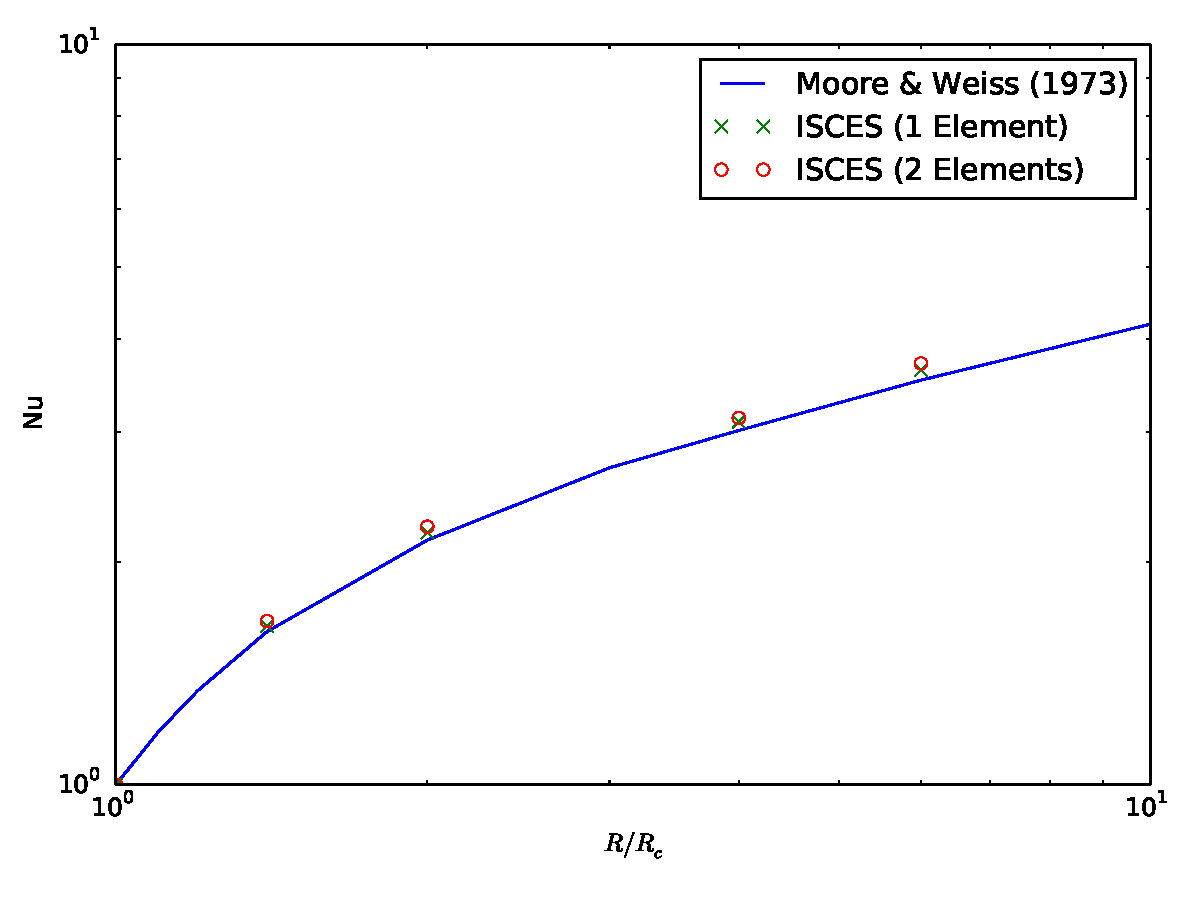
\includegraphics[width=.7\textwidth]{verify.pdf}
	\label{fig:verify}
\end{figure}
}

% \frame{\frametitle{We see near second-order convergence in space and time.}
% \begin{overprint}
% 	\only<1>{
% 		\begin{figure}[h]
% 			\centering
% 				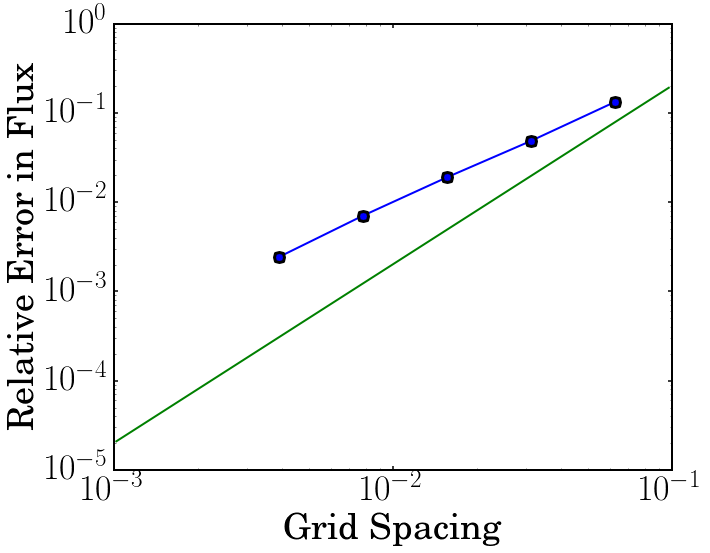
\includegraphics[width=.7\textwidth]{space_convergence.png}
% 			\label{fig:verify}
% 		\end{figure}
% 	}
% 	\only<2>{
% 		\begin{figure}[h]
% 			\centering
% 				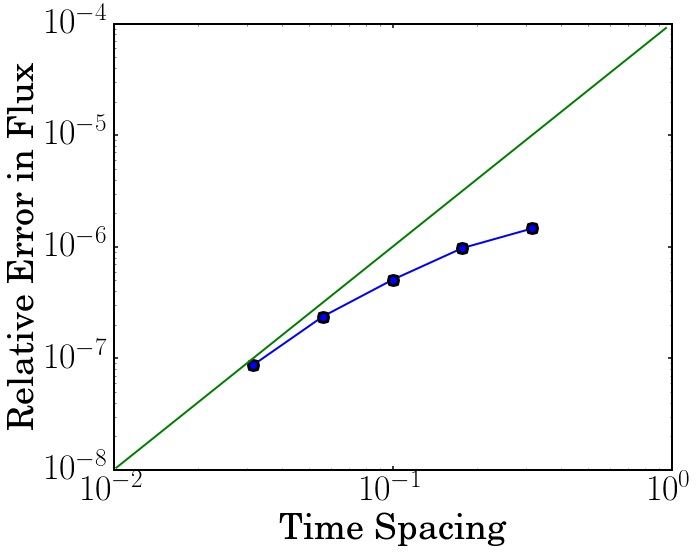
\includegraphics[width=.7\textwidth]{time_convergence.png}
% 			\label{fig:verify}
% 		\end{figure}
% 	}
% \end{overprint}
% }

\frame{\frametitle{We can also compare to the results of the same equations with the same parameters as PADDI.}
\begin{figure}[h]
	\centering
		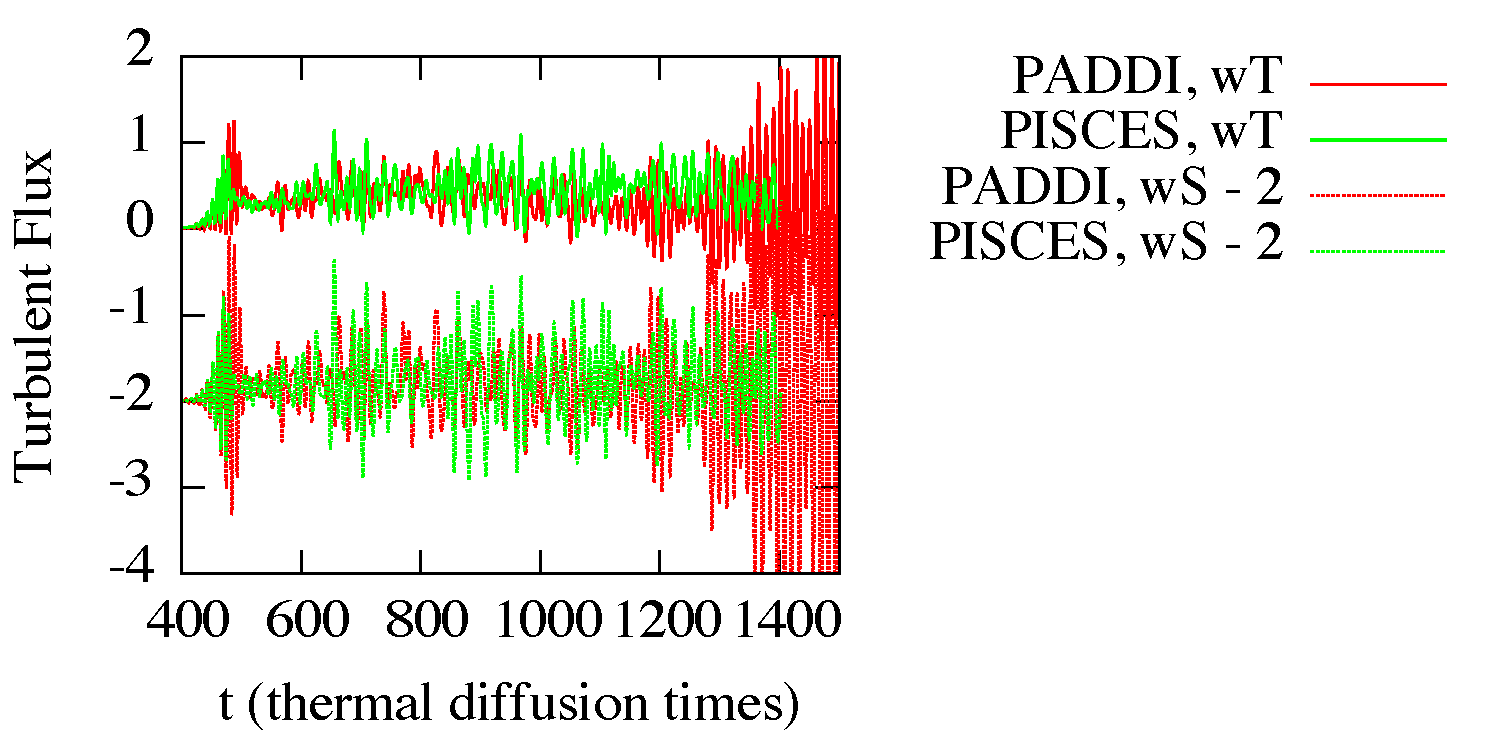
\includegraphics[width=.9\textwidth]{figs/sc_gwave.pdf}
	\caption{The late time behavior is dominated by the boundary conditions, which differ between the codes}
	\label{fig:figs_sc_gwave}
\end{figure}
}